% ====================================================================
%                                                                 
%
%       §01
%
%
% %%ts latex start%%[2019-03-07 Thu 14:45]%%ts latex end%%
% ====================================================================
% --------------------------------------------------------------------
% §1 Section <<Abbildungen>>
% --------------------------------------------------------------------


Im letzten Kapitel haben wir den Begriff der \emph{Menge} eingeführt und einige Konstruktionen damit durchgeführt. Nun möchten wir in der Mathematik nicht nur Mengen an sich betrachten, sondern insbesondere die Zusammenhänge zwischen verschiedenen Mengen. Das zentrale Werkzeug dazu und eine weitere Klasse grundlegender mathematischer Objekte sind die \emph{Abbildungen} zwischen Mengen.




\section{Allgemeines}


\begin{de}
	Seien $X,Y$ zwei Mengen. Eine \textbf{Abbildung} (oder auch \textbf{Funktion}\footnote{Manche Leute bevorzugen das Wort „Abbildung“ im Umfeld abstrakter Mengen und das Wort „Funktion“ im Umfeld von $\Rz$. Wir werden beide Wörter aber völlig synonym verwenden.}) von $X$ nach $Y$ ist eine \emph{Zuordnung} $f$, die jedem Element aus $X$ genau ein Element aus $Y$ zuordnet.
% Bemerkungen Notation
Die Aussage „$f$ ist eine Abbildung von $X$ nach $Y$“ notieren wir kurz und bündig mit:
\begin{align*}
	f:X \to Y \qquad\text{oder auch}\qquad X\xrightarrow{f} Y
\end{align*}
Für ein Element $x \in X$ notieren wir das diesem zugeordnete Element mit
\begin{align*}
 f(x)  && (\text{lies: „$f$ von $x$“})
\end{align*}
und nennen es den \textbf{Funktionswert} von $f$ an der Stelle $x$ oder auch das \emph{Bild} von $x$ unter der Abbildung $f$. Wir schreiben auch
\begin{align*}
 x\mapsto f(x) && (\text{lies: „$x$ geht auf $f(x)$“})
\end{align*}
Die Menge aller Abbildungen von $X$ nach $Y$ notieren wir mit $\text{Abb}(X,Y)$:
\[ \text{Abb}(X,Y) := \{ f \mid f\ \text{ist eine Abbildung von $X$ nach $Y$} \} \]
Ist $f$ eine Abbildung von $X$ nach $Y$, so nennt man die Menge $X$ den \textbf{Definitionsbereich} oder auch die \emph{Quelle} der Abbildung $f$ und die Menge $Y$ den \textbf{Wertebereich} oder auch das \emph{Ziel} der Abbildung $f$.
\end{de}


\begin{bsp}
 \begin{enumerate}[a)]
  \item Wir möchten eine Abbildung $P$ von der Menge aller Katzen $\mathtt{cat}$ in die Menge aller Farben $\mathtt{colour}$ notieren, die jeder Katze ihre Fellfarbe zuordnet.
Dann können wir schreiben:
\begin{align*}
	P: \mathtt{cat} &\to \mathtt{colour} \\
	K &\mapsto (\text{Fellfarbe von } K)
\end{align*}
Das soll bedeuten: $P$ ist diejenige Abbildung von $\mathtt{cat}$ nach $\mathtt{colour}$, die jeder Katze $K$ ihre Fellfarbe zuordnet. Ihr Definitionsbereich ist $\mathtt{cat}$ und ihr Wertebereich ist $\mathtt{colour}$.
\item Durch
\[ g : \Rz \to \Rz\ , \ x \mapsto 3x^2-2x+4 \]
ist eine Abbildung $g$ definiert, die von der Menge $\Rz$ in die Menge $\Rz$ geht und jeder Zahl $x\in \Rz$ die Zahl $3x^2-2x+4$ zuordnet. Sie ist ein Beispiel für eine „Polynomfunktion“, wie du sie aus der Schule kennst. Ihr Wertebereich ist gleich ihrem Definitionsbereich, nämlich die Menge der reellen Zahlen. Beispielsweise ist $g(5) = 3\cdot 25 - 2\cdot 5 + 4 = 69$.
\item Die Abbildung
\[ e : \text{Abb}(\Rz,\Rz) \to \Rz \ ,\ f \mapsto f(2) \]
ordnet jeder Abbildung von $\Rz$ nach $\Rz$ ihren Funktionswert an der Stelle $2$ zu. Ihr Definitionsbereich ist $\text{Abb}(\Rz,\Rz)$ und ihr Wertebereich ist $\Rz$. Für die Funktion $g$ von gerade eben wäre beispielsweise
\[ e(g) = g(2) = 3\cdot 4  - 2\cdot 2  + 4=12 \]
\item Sei $X$ eine beliebige Menge. Die Abbildung
\[ F: X \to \mathcal{P}(X) \ ,\ x \mapsto \{x\} \]
hat als Definitionsbereich $X$, als Wertebereich die Potenzmenge von $X$ und sie ordnet jedem Element $x \in X$ diejenige einelementige Menge zu, die nur aus $x$ besteht. Im Fall $X=\Nz$ wäre beispielsweise $F(4) = \{4\}$.
\item Es seien
\begin{align*}
 A & := \{ a \mid a\ \text{ist eine Tonaufnahme} \} & V & := \{v\mid v \ \text{ist ein Video} \}
\end{align*}
Dann hat man eine Abbildung
\begin{align*}
\text{Extraktion der Tonspur} :\quad V&\to A \\
v & \mapsto (\text{Die Tonspur von $v$})
\end{align*}
die jedes Video auf seine Tonspur abbildet. Beispielsweise würde \href{https://www.youtube.com/watch?v=dQw4w9WgXcQ}{dieses Erklärvideo zu Abbildungen} auf \href{https://archive.org/details/NeverGonnaGiveYouUp}{diese Tonaufnahme} abgebildet werden.
 \end{enumerate}
\end{bsp}


\begin{bem}[Abbildungsvorschrift]
 In den Beispielen gerade eben konnte die Abbildung stets durch eine überschaubare Formel beschrieben werden:
 \begin{align*}
  K & \mapsto (\text{Fellfarbe von $K$}) \\
  x & \mapsto 3x^2-2x+4 \\
  f & \mapsto f(2) \\
  x & \mapsto \{x\} \\
  v & \mapsto (\text{Die Tonspur von $v$})
 \end{align*}
 Solche Ausdrücke nennt man auch \emph{Zuordnungsvorschriften} oder \emph{Abbildungsvorschriften}. Jede Beispiel-Abbildung von gerade eben wurde durch die Angabe ihres Definitionsbereichs, ihres Wertebereichs sowie einer Zuordnungsvorschrift definiert. \\
 Beachte aber, dass nicht jede Abbildung eine einfache Zuordnungsvorschrift haben braucht. Abbildungsvorschriften können beliebig kompliziert sein und manche Abbildungen sind so chaotisch, dass sie gar keiner Abbildungsvorschrift gehorchen. Beispielsweise lässt sich mit metamathematischen Methoden nachweisen, dass es Abbildungen $\Nz \to \{0,1\}$ (also Abfolgen von Nullen und Einsen) geben muss, die so chaotisch sind, dass sie nicht durch eine Abbildungsvorschrift beschreibbar sind.
\end{bem}



\begin{bem}[Abbildungsvorschrift mit Fallunterscheidung]
	Eine gelegentlich benutze Möglichkeit, um Abbildungen anzugeben, ist per Fallunterscheidung. Das sieht folgendermaßen aus:
	\begin{align*}
		f:\mathbb{R} &\to \mathbb{R} \\
		x &\mapsto \left \{ \begin{array}{ll}
		x &\text{ falls } x \geq 0\\
		-x	&\text{ falls } x < 0
		\end{array}	
			 \right.
	\end{align*}
Hier haben wir etwa gerade die Betragsabbildung definiert, die gerade $x$ unverändert lässt, falls $x$ nichtnegativ ist und auf $-x$ schickt, falls $x$ negativ ist. \\
Selbstverständlich gibt es auch Fallunterscheidungen mit mehr als 2 Fällen. \\
Es ist auch geläufig, das 'falls' wegzulassen und zu schreiben
\begin{align*}
	f:\mathbb{R} &\to \mathbb{R} \\
	x &\mapsto \left \{ \begin{array}{ll}
		x & x \geq 0\\
		-x	& x < 0
	\end{array}	
	\right.
\end{align*}
Wichtig ist es, darauf zu achten, Definitionsbereiche nicht widersprüchlich doppelt zu vergeben. Im obigen Beispiel wäre es nicht falsch das \dq  < \dq Zeichen durch ein \dq $\leq$ \dq Zeichen zu ersetzen, dies führt zu keinen Widersprüchen. Ein Ausdruck wie
\begin{align*}
	f:\mathbb{R} &\to \mathbb{R} \\
	x &\mapsto \left \{ \begin{array}{ll}
		1  &x \geq 0\\
		-1 &x \leq 0
	\end{array}	
	\right.
\end{align*}
ergäbe aber keinen Sinn. Denn es müsste hier sowohl $f(0)=1$ als auch $f(0)=-1$ gelten, was den Widerspruch $1=-1$ ergäbe.
\end{bem}		

\begin{bem}[Rigorose Abbildungsdefinition]
	Die hier gegebene Abbildungsdefinition ist kurz und nah an der Denkweise vieler Mathematiker. Streng genommen ist sie aber unfundiert, da in ihr das Wort „Zuordnung“ auftaucht, das vorher nicht definiert wurde. Wie genau sich der Begriff der Abbildung präzise mengentheoretisch definieren lässt, lässt sich beispielsweise \href{https://de.wikipedia.org/wiki/Funktion_(Mathematik)#Mengentheoretische_Definition}{hier} in der Wikipedia nachlesen.
	
\end{bem}
%------------------
% Definition Gleichheit von Abbildungen
\begin{de}[Gleichheit von Abbildungen] \label{abbgleich}
	Seien $X,Y$ Mengen, sowie $f: X \to Y$, $g: X \to Y$ zwei Abbildungen
	zwischen diesen Mengen. Dann definieren wir die \textbf{Gleichheit} von $f$ und $g$ via:
	\begin{align*}
		f = g \qquad:\Leftrightarrow\qquad \forall x \in X: f(x) = g(x)
	\end{align*}
\end{de}



\begin{bem}
Eine Abbildung setzt sich zusammen aus ihrem Definitionsbereich, ihrem Wertebereich und der eigentlichen Zuordnung, die jedem Element des Definitionsbereichs ein Element des Wertebereichs zuordnet. Insofern sind Definitions- und Wertebereich grundlegender Bestandteil einer Abbildung und es ergibt nur Sinn, von der Gleichheit zweier Abbildungen zu sprechen, wenn sie dieselbe Quelle und dasselbe Ziel haben. \\
Abbildungen mit gleicher Zuordnungsvorschrift können sich in Quelle oder Ziel unterscheiden und dann auch sehr unterschiedliche mathematische Objekte sein. Beispielsweise haben die beiden Abbildungen
	\begin{align*}
	 f : \Rz \to \Rz \ & ,\ x\mapsto x^2 \\
	 g : \Zz \to \Nz_0 \ & ,\ x\mapsto x^2
	\end{align*}
	dieselbe Zuordnungsvorschrift, sind aber dennoch zwei verschiedene Abbildungen, da sie verschiedene Definitions- und Wertebereiche haben.
\end{bem}


\begin{bem}[Beweisen, dass zwei Abbildungen gleich oder ungleich sind]
Seien $X,Y$ zwei Mengen. Da die Definition der Gleichheit zweier Abbildungen $f,g:X\to Y$ eine Allaussage ist (für \emph{jedes} $x\in X$ ist $f(x)=g(x)$), kann die Gleichheit $f=g$ nach \cref{allbeweis} dadurch bewiesen werden, dass ein „beliebiges“ Element von $X$ fixiert wird und dann bewiesen wird, dass dessen Funktionswerte unter $f$ und $g$ übereinstimmen. \\
Bevor du überhaupt versuchst, die Gleichheit zweier Abbildungen zu beweisen, solltest du dich natürlich vergewissern, dass sie denselben Definitionsbereich und denselben Wertebereich haben. \\[0.5em]
	Um zu zeigen, dass zwei Abbildungen verschieden sind, genügt es nach \cref{gegenbeispiel}, ein Gegenbeispiel anzugeben, das heißt hier konkret ein Element aus dem Definitionsbereich, das von den zwei Abbildungen auf unterschiedliche Elemente im Zielbereich abgebildet wird. So ein Element zu finden ist nicht immer einfach. Manchmal ist Trial und Error in solchen Fällen hilfreich um Informationen oder Ansätze zu gewinnen.
\end{bem}


\begin{bsp}
	Betrachten wir die Abbildungen: 
	\begin{align*}
		f: \mathbb{R} \to \mathbb{R}\ &,\ x \mapsto x^2 \\
		g: \mathbb{R} \to \mathbb{R}\ &,\ x \mapsto 2x
	\end{align*}
	So ist $f \neq g$, denn $f(1)=1$, aber $g(1)=2$.\\
	Betrachten wir dagegen die Abbildungen:
	\begin{align*}
		\alpha: \Rz \to \mathbb{R}\ &,\ x \mapsto  x^2-1 \\
		\beta: \Rz \to \mathbb{R}\ &,\ x \mapsto (x+1)\cdot (x-1)
	\end{align*}
	so gilt $\alpha=\beta$, denn für jede beliebige reelle Zahl $x\in \Rz$ ist
	\[ \alpha(x) = x^2-1 = (x+1)(x-1) = \beta(x) \]
	sodass sich aus \cref{abbgleich} ergibt, dass $\alpha=\beta$.
\end{bsp}




\section{Bildmengen und Urbildmengen}

%------------------
% Definition Bild- und Urbildabbildung
\begin{de}[Bild und Urbild von Teilmengen] \label{bildmenge}
	Seien $X,Y$ Mengen und $f: X \to Y$ eine Abbildung.
\begin{itemize}
 \item Für eine Teilmenge $A\subseteq X$ heißt
\[ f(A) := \{ f(a) \in Y \mid a\in A \} \]
die \textbf{Bildmenge} oder schlicht das \textbf{Bild} von $A$ unter $f$. 
\item Die Bildmenge von ganz $X$ wird mit $\im(f)$ notiert (für englisch: ``image'')
\[ \im(f) := f(X) = \{y\in Y\mid \exists x\in X:\ f(x)=y  \} \]
und das \textbf{Bild von $f$} genannt.
\item Für eine Teilmenge $B\subseteq Y$ heißt
\[ f^{-1}(B) := \{ x \in X \mid f(x)\in B \} \]
die \textbf{Urbildmenge} oder schlicht das \textbf{Urbild} von $B$ unter $f$.
\item Ist $y\in Y$ irgendein Element, so schreibt man anstelle von „$f^{-1}(\{y\})$“ meist einfach nur „$f^{-1}(y)$“, d.h. bei Urbildern einelementiger Teilmengen lässt man in der Notation die Mengenklammern weg.
\item Die Abbildung, die jeder Teilmenge von $X$ ihre Bildmenge unter $f$ zuordnet
\begin{align*}
 \mathcal{P}(X) \to \mathcal{P}(Y) \ , \ A\mapsto f(A)
\end{align*}
wird meist ebenfalls mit dem Buchstaben „$f$“ bezeichnet (obwohl sie etwas anderes als die Abbildung $f$ ist!) und von uns die \textbf{Bildabbildung} zu $f$ genannt.
\item Die Abbildung, die jeder Teilmenge von $Y$ ihre Urbildmenge unter $f$ zuordnet
\begin{align*}
 \mathcal{P}(Y) \to \mathcal{P}(X) \ , \ B\mapsto f^{-1}(B)
\end{align*}
wird meist mit dem Buchstaben „$f^{-1}$“ bezeichnet und von uns die \textbf{Urbildabbildung} zu $f$ genannt.
\end{itemize}
\end{de}


\begin{bem}
	Man achte darauf, das jetzt mit „$f$“ sowohl die Abbildung selbst als auch die induzierte Abbildung auf den Potenzmengen gemeint sein kann. Die Bedeutung ist also kontextabhängig. Falls man mal den Faden verliert, um welche Abbildung es geht, kann man sich beispielsweise das Argument anschauen, ob es ein Element oder eine Menge ist, und daran erkennen, welche Abbildung man vor sich hat. \\[0.5em]
	Wenn du dich damit besser fühlst, kannst du für dich die Bildabbildung zu $f$ auch mit $\bar{f}$ oder dergleichen notieren; mit der Zeit wirst du dich auch an die doppelte Verwendung des Zeichens „$f$“ gewöhnen.
\end{bem}
\begin{bsp}
	Betrachten wir
	\begin{align*}
    f: \Zz \to \Zz \ ,\ x \mapsto x^2
	\end{align*}
	so gilt z.B.
\begin{align*}
 \im(f) & = \{n\in \Nz_0 \mid n\ \text{ist eine Quadratzahl} \} \\
 f( \{2,-2,6,-5\}) & = \{4,25,36\} \\
 f(\{n\in \Zz \mid n < 0  \}) & = \{n\in \Nz_{\geq 1} \mid n\ \text{ist eine Quadratzahl} \} \\
  f^{-1}(9) & = \{-3,3\} \\
 f^{-1}(\{0,9,16,22\}) & = \{0,3,-3,4,-4\} \\
 f^{-1}(\{2,6,-9\}) & = \emptyset \\
 f^{-1}(\im(f)) & = \Zz
\end{align*}
\end{bsp}

\begin{bsp}[mehr Bilder] \label{bildbsp}
 Es gilt:
 \begin{enumerate}[a)]
  \item Das Bild der Funktion
\[   e : \text{Abb}(\Rz,\Rz) \to \Rz \ ,\ f \mapsto f(2) \]
ist ganz $\Rz$. Denn für jede beliebige reelle Zahl $a\in \Rz$ lässt sich eine „konstante Abbildung“
\[ f_a : \Rz \to \Rz \ ,\  x\mapsto a \]
definieren, die überall den Funktionswert $a$ hat. Dann ist $e(f_a)=f_a(2)=a$ und somit $a\in \im(e)$. Da $a\in \Rz$ beliebig gewählt war, ist somit $\im(e)=\Rz$ bewiesen.
\item Das Bild der Funktion
\[ F: X \to \mathcal{P}(X) \ ,\ x \mapsto \{x\} \]
ist $\{T\in\mathcal{P}(X)\mid T\ \text{enthält genau ein Element} \}$, also die Menge aller einelementigen Teilmengen von $X$.
\begin{bew}
 „$\subseteq$“: Sei $T\in \im(f)$. Dann gibt es ein $x\in X$ mit $T=f(x)=\{x\}$. Also enthält $T$ genau ein Element. \\
 „$\supseteq$“: Sei $T$ eine einelementige Teilmenge von $X$. Da $T$ einelementig ist, gibt es ein Objekt $x$ mit $T=\{x\}$ und da $T$ eine Teilmenge von $X$ ist, ist $x\in X$. Daher ist $f(x)=\{x\}=T$, sodass $T\in \im(f)$ ist. \qed
\end{bew}
\end{enumerate}

\end{bsp}









\section{Verketten}
%------------------
% Definition Komposition von Abbildungen
\begin{de}[Hintereinanderausführung von Abbildungen]\label{verkettung}
	Seien $X,Y,Z$ drei Mengen und $f: X \to Y$, sowie $g: Y \to Z$
	Abbildungen. Mit
	\begin{align*}
	 g\circ f && (\text{lies: „$g$ nach $f$“ oder „$g$ kringel $f$“})
	\end{align*} wird diejenige Abbildung $X\to Z$ bezeichnet, die gegeben ist durch
	\begin{align*}
		g \circ f: X \to Z \ ,\ x \mapsto g(f(x))
	\end{align*}
    Die Abbildung $g\circ f$ heißt die \textbf{Komposition} oder
	\textbf{Verkettung} von $f$ und $g$.
\end{de}



\begin{bem}
 Beachte, dass in der Notation „$g\circ f$“ diejenige Abbildung, die „zuerst“ ausgeführt wird, rechts steht. Für ein Element $x \in X$ berechnet man $(g\circ f)(x)$, indem man zuerst $f(x)$ ausrechnet und darauf nun die Abbildung $g$ loslässt.
\end{bem}


\begin{bsp}
 Betrachte die drei Abbildungen
	\begin{align*}
		f: \mathbb{R} \to \mathbb{R} \ &,\ x \mapsto 2x \\
		g: \mathbb{R} \to \mathbb{R}\ &,\ x \mapsto x^2 \\
		h: \mathbb{R} \to \mathbb{R}\ &,\ x \mapsto 4x^2 
	\end{align*}
Dann gilt für jedes $x\in \Rz$:
\[ (g\circ f)(x) = g(f(x))=g(2x)=(2x)^2 = 4x^2 = h(x) \]
Da $x\in \Rz$ beliebig war, folgt, dass $g\circ f=h$, d.h. $h$ ist genau die Verkettung von $f$ mit $g$.
\end{bsp}



\begin{bsp}[Kommutative Diagramme]
Die Tatsache, dass im letzten Beispiel $g\circ f=h$ gilt, lässt sich visuell auch dadurch ausdrücken, dass „das Diagramm
	\[
	\begin{tikzcd}
		\mathbb{R} \arrow[r, "f"] \arrow[rd,"h"'] &  \arrow[d,"g"] \mathbb{R}  \\ 
		& \mathbb{R}	\end{tikzcd}
	\]
kommutiert“. Dass ein solches Diagramm von Mengen und Abbildungspfeilen kommutiert, besagt, dass es, um von einem Punkt mittels Pfeilen zu einem anderen Punkt zu gelangen, egal ist, welchen Pfad man geht. In diesem Beispiel heißt das also: „Es ist egal, ob ich, um von oben links nach unten rechts zu gelangen, erst die Abbildung $f$ und dann die Abbildung $g$ durchlaufe, oder ob ich stattdessen die Abbildung $h$ durchlaufe“. Und dies ist in unserem Beispiel ja auch tatsächlich egal, da dort $g\circ f=h$ ist.
\end{bsp}





\begin{bem}[Integration durch Substitution]
Die Technik, einer Abbildung $g$ eine Abbildung $f$ „vorzuschalten“, kennst du vielleicht schon aus der Schule als „Variablensubstitution“. In der Methode der „Integration durch Substitution“, die du vielleicht aus der Schule kennst, spielt dies eine maßgebliche Rolle. Sind $f,g:\Rz\to \Rz$ zwei hinreichend „glatte“ Abbildungen und $a,b\in \Rz$, so besagt die Substitutionsregel, dass
 \[ \int_{f(a)}^{f(b)} g = \int_a^b (g\circ f) \cdot f' \]
 Beispielsweise ist
 \begin{align*}
  \int_2^6 x^2\ dx = \int_{2\cdot 1}^{2\cdot 3} x^2\ dx = \int_1^3 (2x)^2 \cdot 2\ dx = 8\cdot \int_1^3 x^2\ dx = 69\tfrac{1}{3}
 \end{align*}
 Falls du diese Methode nicht kennst, ist das nicht schlimm. Sie wird üblicherweise in der Ana1-Vorlesung thematisiert.
\end{bem}



\begin{comment}
\begin{bem}
 Besonders fancy könnte man diesen Satz auch dadurch ausdrücken, dass folgendes Diagramm kommutiert:
 \[ \begin{tikzcd}
 X \ar[r, "\iden_X"] \ar[rd, "f"'] & X \ar[d, "f"]  \ar[rd, "f"] & \\
 & Y \ar[r, "\iden_Y"'] & Y
    \end{tikzcd} \]
 Allerdings ist fraglich, ob die Gleichungen $f\circ \iden_X = f$ und $\iden_Y\circ f=f$ dieselbe Information nicht leichter übermittelt. \\[0.5em]
 Nichtsdestotrotz gibt es (vor allem in der fortgeschrittenen Algebra) viele Situationen, in denen es übersichtlicher ist, ein kommutatives Diagramm zu malen, anstatt Gleichungen von Abbildungen hinzuschreiben. In Situationen, in denen viele Abbildungen auf einmal auftreten, kann dir das Malen eines Diagramms den Überblick erleichtern.
\end{bem}
\end{comment}


\begin{sat}[Verketten von Abbildungen ist assoziativ] \label{abbass}
	Seien $A,B,C,D$ vier beliebige Mengen und $f: A \to B$, $g:B \to C$, $h:C \to D$ drei Abbildungen. Dann gilt:
	\[ h\circ (g\circ f) = (h\circ g)\circ f\]
\end{sat}
\begin{bew}
	Sei $a \in A$ beliebig. Dann gilt 
	\begin{align*}
	(h \circ (g \circ f))(a) & =h ((g \circ f )(a))\\
	& =h(g(f(a))) \\
	& =(h \circ g) (f(a)) \\
	& = ((h \circ g) \circ f) (a)	
	\end{align*}
Da das Element $a\in A$ beliebig gewählt war, folgt mit \cref{abbgleich}, dass $h\circ (g\circ f) = (h\circ g)\circ f$ ist. \qed
\end{bew}


\begin{bem}[Klammern sparen]
 Aufgrund des letzten Satzes kann man in dessen Situation auch einfach
 \[ h\circ g\circ f \]
 schreiben, da es egal ist, ob man erst $g$ mit $f$ verkettet und dann $h$ mit $g\circ f$ -- oder ob man erst $h$ mit $g$ verkettet und dann $f$ mit $h\circ g$. Mit fortgeschrittenen Techniken lässt sich zeigen, dass es auch bei Verkettungen von mehr als drei Abbildungen egal ist, wie man Klammern setzt. Daher werden Klammerungen meist ganz weggelassen.\footnote{vgl. dazu auch \cref{klammerfrei}} Sind etwa $A,B,C,D,E,F$ sechs Mengen und sind Abbildungen
 \[ \begin{tikzcd}
    A \ar[r, "a"] & B \ar[r, "b"] & C \ar[r, "c"] & D \ar[r, "d"] & E \ar[r, "e"] & F
    \end{tikzcd} \]
 gegeben, so notiert man mit
 \[ e\circ d\circ c\circ b\circ a \]
 diejenige Abbildung, die durch Verkettung dieser fünf Abbildungen entsteht, die also daraus besteht, dass man erst $a$ durchläuft, dann $b$, dann $c$, dann $d$ und zuletzt $e$.
\end{bem}






\section{Einschränken}
In diesem Abschnitt seien stets $X,Y$ zwei Mengen und $f:X\to Y$ eine Abbildung. \\

Im folgenden betrachten wir zwei Konstruktionen, mit denen wir die Definitions- und Wertebereiche von Abbildungen verändern können.
\begin{de}[Einschränkung des Definitionsbereichs]
	Sei $X' \subset X$ eine Untermenge von $X$. Dann ist die \textbf{Einschränkung} in der Quelle von $f$ auf $X'$ gegeben durch
	\begin{align*}
		{f|}_{X'}:X' &\to Y\\
		x &\mapsto f(x)
	\end{align*}
Die Zuordnung von $f\vert_{X'}$ funktioniert also genau wie die von $f$, mit dem einzigen Unterschied, dass der Definitionsbereich verkleinert wurde und $f\vert_{X'}$ nur noch den Elementen aus $X'$ etwas zuordnet.
\end{de}



\begin{bsp}
 Betrachte die Abbildung
 \[ f : \Rz \to \Rz \ ,\ x \mapsto x^2-2 \]
 Deren Einschränkung auf die Teilmenge $\Qz\subseteq \Rz$ ist dann gegeben durch
 \[ f\vert_{\Qz} : \Qz \to \Rz \ ,\ x\mapsto x^2-2 \]
 Obwohl die Zuordnungsvorschrift ($x\mapsto x^2-2)$ dieselbe ist, handelt es sich um eine andere Funktion! Beispielsweise ist $f^{-1}(0)= \{\sqrt{2},-\sqrt{2}\}$, d.h. die Funktion $f$ besitzt genau zwei Nullstellen. Dagegen ist $(f\vert_{\Qz})^{-1}(0) = \emptyset$, d.h. die Funktion $f\vert_{\Qz}$ besitzt keine Nullstelle.
\end{bsp}



\begin{de}[Einschränkung des Wertebereichs]\label{zielschrank}
	Ist $\im(f) \subset Y' \subset Y$ eine Zwischenmenge des Bildes von $\im(f)$ und $Y$, so können wir die \textbf{Einschränkung} von $f$ auf $Y'$ betrachten:
	\begin{align*}
		f|^{Y'}:X &\to Y'\\
		x &\mapsto f(x)
	\end{align*}
Die Zuordnung von $f\vert_{X'}$ funktioniert also genau wie die von $f$, mit dem einzigen Unterschied, dass der Wertebereich von $f$ verkleinert wurde. Ist $x\in X$, so ist zwar $f\vert^{Y'}(x) = f(x)$, allerdings liegt bei $f(x)$ die Betonung darauf, dass es sich um ein Element von $Y$ handelt, während bei $f\vert^{Y'}(x)$ die Betonung darauf liegt, dass es sich um ein Element von $Y'$ handelt.
\end{de}



\begin{bsp}
Es seien $M := \{ x\mid x\ \text{steht in der Startelf des FC Bayern} \}$ sowie
\[ f : M \to \Rz \ ,\ x \mapsto (\text{Das Jahresgehalt von $x$}) \]
Dann ist $\im(f)\subseteq \Rz_{\geq 5.000.000}$, da (Stand 2021/22) jeder Spieler in der Startelf der Bayern ein Jahresgehalt von über fünf Millionen Euro bezieht\footnote{Quelle: \href{https://www.vermoegenmagazin.de/bayern-muenchen-gehaelter/}{vermoegenmagazin.de}. Beachte, dass die realen Einkommen dank Prämien und Werbeverträgen nochmal deutlich höher sind.}. Also lässt sich der Wertebereich von $f$ auf $\Rz_{\geq 5.000.000}$ einschränken, wodurch man die Abbildung
\[ f : M \to \Rz_{\geq 5.000.000} \ ,\ x \mapsto (\text{Das Jahresgehalt von $x$}) \]
erhält.
\end{bsp}



\begin{bem}
 Beachte, dass sich der Wertebereich einer Funktion $f$ nur auf solche Teilmengen einschränken lässt, die $\im(f)$ umfassen. Ist beispielsweise
  \[ f : \Rz \to \Rz \ ,\ x \mapsto x^2-2 \]
so ergäbe der Ausdruck „$f\vert^{\Qz}$“ keinen Sinn. Denn der Ausdruck
\begin{align*}
 \text{„$f\vert^{\Qz} : \Rz \to \Qz \ ,\ x\mapsto x^2-2$“} && (\text{Dies ergibt keinen Sinn})
\end{align*}
definiert keine Abbildung, da etwa $f(\sqrt{\pi + 2})$ gar kein Element von $\Qz$ ist. \\[0.5em]
Im Gegensatz zum Wertebereich einer Funktion lässt sich deren Definitionsbereich aber problemlos auf beliebige Teilmengen einschränken.
\end{bem}







\section{Besondere Abbildungen}


%------------------
% Definition Identitaetsabb.


\subsection{Identität}
Sei $X$ eine beliebige Menge. Gibt es überhaupt eine Abbildung $X\to X$? Solange wir nicht mehr Informationen über die Elemente von $X$ haben, können wir ja schwerlich eine besondere Abbildungsvorschrift angeben. Dennoch gibt es stets eine Abbildung $X\to X$, deren Zuordnungsvorschrift so simpel ist, dass man sie schon wieder übersehen kann:

\begin{de}[Identitätsabbildung]
	Sei $X$ eine Menge. Die Abbildung
	\begin{align*}
		\iden_X: X &\to X \\
		x &\mapsto x
	\end{align*}
	heißt die \textbf{Identität auf $X$}.
\end{de}

\begin{bem}
Die Identität auf der Menge $X$ bildet also jedes Element aus sich selbst ab und „lässt alles unverändert“. Die Identität auf $\Rz$ kennt ihr auch schon aus der Schule: die Polynomfunktion „$f(x)=x$“ ist genau die Identitätsabbildung $\iden_{\Rz}$ auf der Menge der reellen Zahlen.
\end{bem}



Die Identität ist eine sehr wichtige Abbildung, denn sie wirkt hinsichtlich der Verkettung von Abbildungen gewissermaßen wie die $0$ bei der Addition oder die $1$ bei der Multiplikation:\footnote{vgl. \cref{neutrales}}
\begin{sat}[Neutralität der Identität] \label{idneutral}
    Seien $X,Y$ zwei beliebige Mengen und $f:X\to Y$ eine Abbildung von $X$ nach $Y$. Dann gilt:
    \begin{align*}
     f\circ \iden_X & = f \\
     \iden_Y \circ f & = f
    \end{align*}
\end{sat}
\begin{bew}
	Ist $x \in X$ ein beliebiges Element, so gilt
    \begin{align*}
(f\circ \iden_X)(x) & = f(\iden_X(x)) \\
    & =f(x) && (\text{Definition von $\iden_X$}) \\
(\iden_Y \circ f)(x) & =\iden_Y(f(x)) \\
& = f(x)&& (\text{Definition von $\iden_Y$})
\end{align*}
Da das Element $x\in X$ beliebig gewählt war, folgen die Gleichungen $f\circ \iden_X=f$ und $\iden_X\circ f=f$ mit \cref{abbgleich}. \qed
\end{bew}




\subsection{Inklusion einer Teilmenge}

\begin{de}[Inklusionsabbildung]
	Sei $A,B$, zwei Mengen, wobei $A$ eine Untermenge von $B$ sei. Dann haben wir die sogenannte (natürliche) \textbf{Inklusion}, meist notiert mit dem griechischen Buchstaben $\iota$ (Iota):
	\begin{align*}
		\iota: A \to B \ ,\ a \mapsto a
	\end{align*}
Die natürliche Inklusion ordnet einem Element aus $A$ genau das gleiche Element in $B$ zu. Genauso wie bei der Identitätsabbildung wird auch von der Inklusion „nichts verändert“. Allerdings bewirkt die Inklusion eine „Kontextverschiebung“. Ist $a\in A$ irgendein Objekt, von dem betont ist, dass es ein Element von $A$ ist, so ist $\iota(a)$ nachwievor dasselbe Objekt, jetzt aber betont als Element von $B$.
\end{de}



\begin{bsp}
 Da $\Zz$ eine Teilmenge von $\Qz$ ist, hat man die Inklusionsabbildung $\Zz \to \Qz$, die jede ganze Zahl auf sich selbst, nun aufgefasst als rationale Zahl, abbildet.
\end{bsp}
So wirklich interessante Beispiele fallen uns hierzu auch nicht ein -- denn die Inklusion „tut ja nichts“, außer den Kontext der Elemente erweitern.





\begin{bem}[„Kanonizizät“ der natürlichen Inklusion]
 Seien $X$ eine beliebige Menge und $U\subseteq X$ eine Teilmenge. Spricht man ohne weitere Spezifikation von „der Abbildung $U\to X$“, so ist damit meistens die natürliche Inklusion gemeint. Denn welche „natürliche“ Abbildung sollte es, sofern dir keine weiteren Informationen über $X$ und $U$ bekannt sind, außer dass halt $U$ eine Teilmenge von $X$ ist, sonst noch von $U$ nach $X$ geben? \\
 Darin besteht das „Natürliche“ an der natürlichen Inklusion: dass man völlig unabhängig von der konkreten Gestalt von $X$ und der Teilmenge $U$ stets eine konkrete Abbildung $U\to X$ zur Hand hat, nämlich die Inklusion.
\end{bem}




\begin{sat}
 Seien $X,Y$ zwei beliebige Mengen, $f:X\to Y$ eine Abbildung , $U\subseteq X$ irgendeine Teilmenge von $X$ und $\iota_U : U\to X$ die natürliche Inklusion. Dann gilt:
 \[ f\vert_U = f\circ \iota_U \]
 d.h. die Einschränkung von $f$ auf $U$ lässt sich dadurch erhalten, dass man $f$ mit $\iota_U$ verkettet.
\end{sat}
\begin{bew}
 Wegen $f\in \text{Abb}(X,Y)$ und $\iota_U \in \text{Abb}(U,X)$ ist $f\circ \iota_U$ eine Abbildung von $U$ nach $X$, genauso wie $f\vert_U$. Also stimmen schonmal Definitions- und Wertebereich überein. Da außerdem für jedes beliebige $x\in U$ gilt:
 \[ (f\circ \iota_U)(x) = f(\iota_U(x)) = f(x) = f\vert_U(x) \]
 gilt insgesamt die Gleichheit von Abbildungen $f\vert_U = f\circ \iota$. \qed
\end{bew}



\begin{bem}
Insbesondere ist
\[ \iden_X \vert_U = \iden_X \circ \iota_U =  \iota_U\]
d.h. die Inklusion von $U$ in $X$ ist genau die Einschränkung der Identität $\iden_X$ auf die Teilmenge $U$.
\end{bem}







\subsection{Umkehrabbildungen}
In diesem Abschnitt seien stets $X,Y$ zwei Mengen und $f:X\to Y$ eine Abbildung.

\begin{de}[Umkehrabbildung] \label{umkehrabb}
Eine Abbildung $g:Y \to X$ heißt \textbf{Umkehrabbildung von $f$} oder auch eine \textbf{inverse Abbildung zu $f$}, falls sie die beiden „Inversengleichungen“ erfüllt:
	\begin{align*}
    g \circ f &= \iden_X, \\
    f \circ g &= \iden_Y.
	\end{align*}
Falls $f$ eine Umkehrabbildung besitzt, nennt man $f$ eine \textbf{invertierbare Abbildung}.
\end{de}



\begin{bsp}
Die Abbildung
\[f : \Rz_{>-1} \to \Rz_{>0} \ ,\ x \mapsto \frac{1}{x+1} \]
ist invertierbar, denn die Abbildung
\[g: \Rz_{>0} \to \Rz_{>-1} \ ,\ x \mapsto \frac{1}{x} -1 \]
ist eine Umkehrabbildung.
\end{bsp}
Die Abbildung $g$ habe ich dadurch gefunden, dass ich die Gleichung $y= \frac{1}{x+1}$ nach $y$ umgestellt habe.
\begin{bew}
 ($g\circ f = \iden$): Für jede Zahl $x\in \Rz_{>-1}$ ist
 \begin{align*}
 (g\circ f)(x) & = g(f(x)) \\
 & = g\left(\frac{1}{x+1}\right) \\
 & = \frac{x+1}{1} - 1 \\
 & = x = \iden_{\Rz_{>-1}}(x)
 \end{align*}
Da $x\in \Rz_{>0}$ beliebig war, folgt die Gleichheit von Abbildungen $g \circ f= \iden_{\Rz_{>-1}}$. \\[0.5em]
 ($f\circ g = \iden$): Sei $y\in \Rz_{>0}$ beliebig. Dann gilt
 \begin{align*}
  (f\circ g)(y) & = f(g(y)) \\
  & = f\left( \frac{1}{y} -1\right) \\
  & = \frac{1}{\left(\frac{1}{y} -1\right) +1} \\
  & = \frac{1}{\frac{1}{y}} \\
  & = y = \iden_{\Rz_{>0}}(y)
 \end{align*}
 und da $y\in \Rz$ beliebig war, folgt die Gleichheit von Abbildungen $f\circ g = \iden_{\Rz_{>0}}$. \qed
\end{bew}








\begin{sat}[Eindeutigkeitssatz für inverse Abbildungen]\label{umkehreind}
Wenn $f$ eine invertierbare Abbildung ist, so gibt es auch nur \emph{genau eine} Umkehrabbildung zu $f$.\footnote{vgl. \cref{inveind}}
\end{sat}
\begin{bew}
 Seien $g,h:Y\to X$ zwei inverse Abbildungen zu $f$. Dann gilt:
 \begin{align*}
  g & = g\circ \iden_Y && (\text{nach \cref{idneutral}})\\
  & = g\circ (f\circ h) && (\text{da $h$ invers zu $f$ ist}) \\
  & = (g\circ f)\circ h && (\text{nach \cref{abbass}}) \\
  & = \iden_X \circ h && (\text{da $g$ invers zu $f$ ist}) \\
  & = h && (\text{nach \cref{idneutral}}) 
 \end{align*}
Also ist die Umkehrabbildung $f$ eindeutig bestimmt. \qed
\end{bew}


\begin{bem}[\textbf{Die} Umkehrabbildung]
Der letzte Satz berechtigt uns dazu, anstelle von „einer Umkehrabbildung von $f$“ von \emph{der} Umkehrabbildung von $f$ zu sprechen. \\
Die inverse Abbildung zu $f$ notiert man meistens mit
\[ f^{-1} \]
Beachte nochmal, dass es nur nur dann Sinn ergibt, von der „Umkehrabbildung $f^{-1}$“ zu sprechen, wenn $f$ invertierbar ist. Wir werden in \cref{invwiderleg} Techniken kennenlernen, mit denen sich beweisen lässt, dass eine Abbildung nicht invertierbar ist.
\end{bem}



\begin{comment}
\begin{sat} \label{idinvertierbar}
 Sei $X$ eine beliebige Menge. Dann ist $\iden_X$ eine invertierbare Abbildung und es ist $\iden_X^{-1}=\iden_X$.
\end{sat}
\begin{bew}
 Nach \cref{idneutral} ist
 \[ \iden_X\circ \iden_X = \iden_X \]
 Und damit gelten bereits beide Inversengleichungen aus \cref{umkehrabb}. 
\end{bew}
\end{comment}





\begin{bem}
Das Zeichen „$f^{-1}$“ ist bereits in \cref{bildmenge} aufgetaucht und wurde dort im Kontext von Urbildmengen benutzt. Sofern $f$ eine invertierbare Abbildung ist, bezeichnet „$f^{-1}$“ also zwei verschiedene Abbildungen auf einmal: die inverse Abbildung $f^{-1}:Y\to X$ sowie die Urbildabbildung $f^{-1} : \mathcal{P}(Y)\to \mathcal{P}(X)$. \\[0.5em]
Hier ist eine Tabelle mit den verschiedenen Bedeutungen von „$f$“ und „$f^{-1}$“:
\[ \begin{tabular}{L|L}
    \text{Zeichen} & \text{Bedeutung} \\ \hline 
    f & \text{Die Abbildung}\ X \to Y \ ,\ x \mapsto f(x) \\
    f & \text{Die (mengenwertige) Abbildung}\ \mathcal{P}(X) \to \mathcal{P}(Y) \ ,\ A\mapsto f(A)  \\
    f^{-1} & \text{Die (mengenwertige) Abbildung}\ \mathcal{P}(Y) \to \mathcal{P}(X) \ ,\ B\mapsto f^{-1}(B) \\
    f^{-1} & \text{Die (mengenwertige) Abbildung}\ Y \to \mathcal{P}(X) \ ,\ y\mapsto f^{-1}(y) \\ \hline
    f^{-1} & \text{Die Umkehrabbildung}\ f^{-1} : Y\to X \ ,\ y \mapsto f^{-1}(y) \\
    & (\text{existiert nur, sofern $f$ invertierbar ist}) 
   \end{tabular} \]
Beachte, dass die ersten vier Abbildungen immer existieren; die fünfte Abbildung aber nur dann, wenn $f$ invertierbar ist.	
%Wie wir oben gesehen haben, ist beispielsweise die Abbildung $f: \mathbb{R} \to \mathbb{R}, x \to x^2$ nicht bijektiv, hat also keine Umkehrabbildung. Wohl aber existiert die Urbildabbildung, die jeder positiven reellen Zahl, die Menge die die Zahl selbst und ihr Negatives enthält zuordnet und jeder negativen reellen Zahl die leere Menge.
\end{bem}



\subsection{Projektionen beim kartesischen Produkt}
\begin{de}
	Seien $X,Y$ zwei Mengen. Die Abbildungen
	\begin{align*}
		{\pi}_1 :X \times Y &\to X \\
		(x,y) &\mapsto x \\	
		{\pi}_2 :X \times Y &\to Y \\
		(x,y) &\mapsto y 
	\end{align*}
heißen \textbf{kanonischen Projektionen}.
\end{de} 

\begin{bsp}
 Interpretiert man $\Rz^2=\Rz\times \Rz$ als die Menge der „Punkte in der Ebene“, so kann man sich die beiden Projektionen $\Rz\times \Rz \to \Rz$ als „Orthogonalprojektionen auf die Koordinatenachsen“ vorstellen, die jeden Punkt in der Ebene auf seine x-Koordinate bzw. seine y-Koordinate abbilden.
     \begin{figure}[H]
\begin{center}
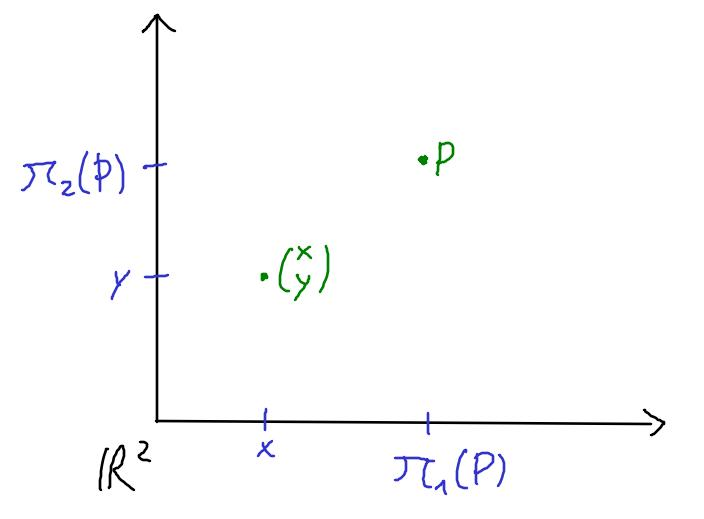
\includegraphics[width=10cm]{./_img/Projektion.jpeg}
\end{center}
\centering \caption{x-Koordinate und y-Koordinate eines Punkts in der Ebene}
\end{figure}
\end{bsp}

\begin{bem}[Komponentenweises Definieren von Abbildungen]
Seien $A,X,Y$ drei Mengen. Eine Abbildung $A\to X\times Y$ lässt sich „komponentenweise definieren“, sofern man eine Abbildung $A\to X$ und eine Abbildung $A\to Y$ zur Hand hat. \\
Um genau zu sein: Sind $f:A\to X$ und $g:A\to Y$ zwei Abbildungen, so erhält man eine Abbildung
\[ A \to X\times Y \ ,\ a \mapsto (f(a),g(a)) \]
die „in der ersten Komponente“ durch $f$ und „in der zweiten Komponente“ durch $g$ gegeben ist. Insgesamt liefert diese Technik eine Abbildung
\begin{align*}
  \text{Abb}(A,X)\times \text{Abb}(A,Y) & \to \text{Abb}(A,X\times Y) \\
  (f,g) & \mapsto (a \mapsto (f(a),g(a))
\end{align*}
\end{bem}

\begin{bsp}
 Die beiden Abbildungen
 \begin{align*}
  f : \Rz^2 \to \Rz \ &,\ (x,y) \mapsto 3x-y \\
  g : \Rz^2 \to \Rz \ &,\ (x,y) \mapsto 4x
 \end{align*}
können kombiniert werden zur Abbildung
\[ \Rz^2 \to \Rz^2 \ ,\ (x,y) \mapsto (f(x,y),g(x,y)) = (3x-y,4x) \]
die in der ersten Komponente durch $f$ und in der zweiten Komponente durch $g$ gegeben ist. Aus der Schule weißt du vielleicht schon, dass man diese Abbildung durch eine Matrix darstellen kann:
\[ \begin{pmatrix}
    x \\ y
   \end{pmatrix} \mapsto \begin{pmatrix}
   3 & -1 \\
   4 & 0
   \end{pmatrix} \cdot \begin{pmatrix}x \\ y   \end{pmatrix}\]
\end{bsp}








\section{Injektiv, surjektiv, bijektiv}

Wir schauen uns nun einige grundlegende Eigenschaften an, die Abbildungen besitzen können. Um zu vermitteln, dass es nicht immer die eine richtige Definition gibt, geben wir diese über äquivalente Bedingungen an. Der Kniff in der Anwendung ist es dann, jeweils jene zu finden die im Augenblick am praktischsten ist. Dies ist oft auch Geschmackssache.
\begin{de}[Injektive Abbildung] \label{injektiv}
	Seien $X, Y$ Mengen und $f: X \longra Y$ eine Abbildung. Dann sind
	äquivalent
	\begin{enumerate}[(i)]
		\item  Für alle $x_{1},x_{2} \in X$ mit $x_1\neq x_2$ gilt $f(x_1)\neq f(x_2)$.
		\item Für alle $x_{1},x_{2}\in X$ mit $f(x_{1})=f(x_{2})$ gilt
		bereits $x_{1}=x_{2}$.
		\item Für alle $y\in Y$ ist die Urbildmenge $f^{-1}(y)$ höchstens
		einelementig.
	\end{enumerate}
Erfüllt $f$ eine (und damit alle) dieser drei äquivalenten Bedingungen, so heißt $f$ eine \textbf{injektive} Abbildung.
\end{de}
\begin{bew}
	\begin{itemize}
		\item[(i)$\Leftrightarrow$(ii)] Es ist (i) genau die Kontraposition von (ii) und damit zu (ii) äquivalent.
		\item[(ii)$\Rightarrow$(iii)] Seien $y\in Y$ und $x_{1},x_{2}\in f^{-1}(y)$. Dann gilt $f(x_{1})
		= y = f(x_{2})$, also wegen $(ii)$ bereits $x_{1}=x_{2}$. Damit ist bewiesen, dass $f^{-1}(y)$ höchstens einelementig ist. Da $y\in Y$ beliebig gewählt war, folgt (iii).
		\item[(iii)$\Rightarrow$(ii)] Seien $x_1,x_2\in X$ mit $f(x_1)=f(x_2)$. Für $y:= f(x_1)$ gilt dann $x_1,x_2\in f^{-1}(y)$. Da $f^{-1}(y)$ nach (iii) aber nur höchstens einelementig ist, muss dann $x_1=x_2$ gelten. \qed
	\end{itemize}
\end{bew}

\begin{bsp} Es gilt:
\begin{enumerate}[a)]
 \item Die Abbildung
 \[ f: \mathbb{R} \to \mathbb{R}\ ,\ x \mapsto x^2 \]
 ist nicht injektiv, da beispielsweise $f(-2)=f(2)$, aber $-2 \neq 2$.
 \item Die Abbildung
 \[ e: \text{Abb}(\Rz,\Rz) \to \mathbb{R}\ ,\ f \mapsto f(2)\]
 ist nicht injektiv. Betrachte dazu die beiden Abbildungen
 \begin{align*}
  f : \Rz \to \Rz \ &,\  x\mapsto x+2 \\
  g : \Rz \to \Rz \ &,\  x\mapsto 2x
 \end{align*}
 Wegen $f(1)\neq g(1)$ ist $f\neq g$ aber es ist dennoch
 \[ e(f)=f(2)=4=g(2)=e(g) \]
 \item Sei $X$ eine beliebige Menge. Die Abbildung
 \[ F : X \to \mathcal{P}(X) \ ,\ x \mapsto \{x\} \]
 ist injektiv. Denn sind $x,y\in X$ beliebig mit $F(x)=F(y)$, so ist
 \[ x\in \{x\} = F(x) = F(y) = \{y\} \]
 sodass $x=y$ sein muss. Da die Elemente $x,y\in X$ beliebig gewählt waren, folgt aus (ii) von \cref{injektiv}, dass $F$ injektiv ist.
 \item Sind $X$ eine beliebige Menge, $U\subseteq X$ eine Teilmenge und $\iota : U\to X$ die natürliche Inklusion, so ist $\iota$ eine injektive Abbildung. Denn sind $x,y\in U$ mit $\iota(x)=\iota(y)$, so ist bereits $x=y$, da ja $\iota(x)=x$ und $\iota(y)=y$ gilt.
\end{enumerate}
\end{bsp}
	

\begin{de}[Surjektive Abbildung] \label{surjektiv}
	Seien $X, Y$ Mengen und $f: X \to Y$ eine Abbildung. Dann sind
	äquivalent:
	\begin{enumerate}[(i)]
		\item Für alle $y\in Y$ existiert ein $x\in
		X$, sodass $f(x)=y$.
                \item Es gilt $\im(f) = Y$, d.h. das Bild von $f$ stimmt mit seinem Wertebereich überein.
		\item Für alle $y\in Y$ ist die Urbildmenge $f^{-1}(\{ y \})$ mindestens
		einelementig.
	\end{enumerate}
	Erfüllt $f$ eine (und damit alle) dieser drei äquivalenten Bedingungen, so heißt $f$ eine \textbf{surjektive} Abbildung.
\end{de}

%------------------
% Beweis
\begin{bew}
	\begin{itemize}
    \item[(i)$\Leftrightarrow$(ii)] Per Definition von $\im(f)$ ist
    \[ \im(f) = \{y\in Y\mid \exists x\in X:\ f(x)=y \} \]
    Also ist genau dann $\im(f)=Y$, wenn es für jedes Element $y\in Y$ ein $x\in X$ mit $f(x)=y$ gibt.
		\item[(i)$\Leftrightarrow$(iii)] 
    Für jedes $y\in Y$ ist:
    \[ f^{-1}(y) = \{x\in X\mid f(x)=y \} \]
    Dass $f^{-1}(y)$ mindestens ein Element enthält, besagt also gerade, dass es mindestens ein $x\in X$ mit $f(x)=y$ gibt. Da dies für jedes $y\in Y$ gilt, folgt die Äquivalenz (i)$\Leftrightarrow$(iii). \qed
	\end{itemize}
\end{bew}





\begin{bsp}
Es gilt:
\begin{enumerate}[a)]
 \item Die Abbildung
 \[ f:\mathbb{N}_0 \to \mathbb{N}_0 \ ,\ n \mapsto n+1 \]
 ist nicht surjektiv. Denn es gibt keine natürliche Zahl $n\in \Nz_0$, für die $0=f(n)=n+1$ gälte. Daher ist $0\notin \im(f)$ und $f$ ist nicht surjektiv.
  \[ \begin{tikzcd}
 f: & 0 \ar[r, bend left, mapsto]& 1 \ar[r, bend left, mapsto]& 2 \ar[r, bend left, mapsto]& 3 \ar[r, bend left, mapsto]& 4 \ar[r, bend left, mapsto]& 5 \ar[r, bend left, mapsto]& \dots
    \end{tikzcd} \]
 \item Die Abbildung
 \[ g: \mathbb{N}_0 \to \mathbb{N}_0\ ,\ n \mapsto \begin{cases}
n-1 & n\geq 1 \\
0 & n=0
\end{cases}  \]
 hingegen ist surjektiv, denn für jedes $n \in \mathbb{N}_0$ ist $n+1\in g^{-1}(n)$.
 \[ \begin{tikzcd}
g: & 0  & 1 \ar[l, bend right, mapsto] & 2 \ar[l, bend right, mapsto] & 3 \ar[l, bend right, mapsto] & 4  \ar[l, bend right, mapsto] & 5  \ar[l, bend right, mapsto] &  \ar[l, bend right, mapsto]  \dots
    \end{tikzcd} \]
 \item Die Abbildung
 \[ e : \text{Abb}(\Rz,\Rz) \to \Rz \ ,\ f\mapsto f(2) \]
 ist surjektiv, was bereits in \cref{bildbsp} gezeigt wurde.
 \item Ist $X$ eine beliebige Menge, so ist die Abbildung
 \[ F : X\to \mathcal{P}(X) \ ,\ x\mapsto \{x\} \]
 nicht surjektiv. Denn das Bild von $F$ besteht aus genau den einelementigen Teilmengen von $X$, aber nicht jede Teilmenge von $X$ ist einelementig. Z.B. ist $\emptyset\subseteq X$ eine nullelementige Teilmenge.
\end{enumerate}
\end{bsp}





\begin{de}[Bijektive Abbildung] \label{bijektiv}
	Eine Abbildung heißt \textbf{bijektiv}, wenn sie sowohl injektiv als auch surjektiv ist.
\end{de}



\begin{bem}
 Seien $X,Y$ zwei Mengen und $f:X\to Y$ eine Abbildung. Nach \cref{injektiv} und \cref{surjektiv} gilt
 \begin{align*}
  f\ \text{ist injektiv}\qquad &\Leftrightarrow\qquad \text{Für jedes $y\in Y$ enthält $f^{-1}(\{y\})$ höchstens ein Element} \\
    f\ \text{ist surjektiv}\qquad &\Leftrightarrow\qquad \text{Für jedes $y\in Y$ enthält $f^{-1}(\{y\})$ mindestens ein Element}
 \end{align*}
Also ist $f$ genau dann bijektiv, wenn für jedes $y\in Y$ die Urbildmenge $f^{-1}(\{y\})$ aus \emph{genau einem} Element besteht.
\end{bem}



\begin{sat}[Bijektiv $\Leftrightarrow$ invertierbar] \label{invkriterium}
Seien $X,Y$ zwei Mengen und $f:X\to Y$ eine Abbildung. Dann sind äquivalent:
\begin{enumerate}[(i)]
 \item $f$ ist eine bijektive Abbildung.
 \item $f$ ist eine invertierbare Abbildung.
\end{enumerate}
\end{sat}
\begin{bew}
 (i)$\Rightarrow$(ii): Sei $f$ bijektiv. Für jedes $y\in Y$ enthält dann die Urbildmenge $f^{-1}(\{y\})$ genau ein Element. Definiere die Abbildung
 \[ g : Y\to X \ ,\ y \mapsto (\text{Das eine Element von $f^{-1}(\{y\})$}) \]
 Dann ist $g$ invers zu $f$, denn: \\
 ($g\circ f=\iden_X$) Für ein beliebiges $x\in X$ ist
 \begin{align*}
  (g\circ f)(x) & = g(f(x)) \\
  & = (\text{Das eine Element von $f^{-1}(\{f(x)\})$}) \\
  & = x && (\text{da $f(x)\in \{f(x)\}$}) \\
  & = \iden_X(x)
 \end{align*}
 Weil $x\in X$ beliebig war, folgt die Gleichheit von Abbildungen $g\circ f=\iden_X$. \\[0.5em]
 ($f\circ g=\iden_Y$) Für ein beliebiges $y\in Y$ ist
  \begin{align*}
  (f\circ g)(y) & = f(\text{Das eine Element von $f^{-1}(\{y\})$}) \\
  & = y && (\text{per Definition von $f^{-1}(\{y\})$}) \\
  & = \iden_Y(y)
 \end{align*}
 Also ist $f\circ g=\iden_Y$. Insgesamt ist damit gezeigt, dass $g$ invers zu $f$ ist. \\[0.5em]
 (ii)$\Rightarrow$(i): Sei $f$ invertierbar und sei $f^{-1}:Y\to X$ die inverse Abbildung. Dann ist $f$ bijektiv, denn: \\
 (Injektivität): Seien $x,y\in X$ mit $f(x)=f(y)$. Es folgt
 \begin{align*}
   x & = f^{-1}(f(x)) && (\text{da $f^{-1}\circ f=\iden_X$})\\
   & = f^{-1}(f(y)) &&  (\text{da $f(x)=f(y)$}) \\
   & = y  &&  (\text{da $f^{-1}\circ f=\iden_X$})
 \end{align*}
 Da $x,y\in X$ beliebig waren, ist bewiesen, dass $f$ injektiv ist. \\
 (Surjektivität): Sei $y\in Y$ beliebig. Dann ist
 \begin{align*}
  y & = f(f^{-1}(y)) && (\text{da $f\circ f^{-1}=\iden_Y$}) \\
  & \in \im(f)
 \end{align*}
Da das Element $y\in Y$ beliebig war, ist damit bewiesen, dass $\im(f)=Y$, also dass $f$ surjektiv ist.\qed
\end{bew}





\begin{bem}[Bijektivität beweisen]
 Ist $f$ eine Abbildung, für die du beweisen möchtest, dass sie bjektiv ist, so stehen dir damit zwei Wege offen:
 \begin{enumerate}
  \item Du arbeitest mit \cref{bijektiv}, d.h. du beweist sowohl, dass $f$ injektiv ist, als auch, dass $f$ surjektiv ist.
  \item Du arbeitest mit \cref{invkriterium}, d.h. du schreibst einen Kandidaten für die Umkehrabbildung hin und beweist daraufhin, dass er tatsächlich invers zu $f$ ist.
 \end{enumerate}
Es gibt Situationen, wo es schwer bis unmöglich ist, eine konkrete Abbildungsvorschrift für eine Umkehrabbildung anzugeben. In diesem Fall ist der erste Weg leichter. \\
Es gibt aber auch Situationen, in denen du unmittelbar „siehst“, dass $f$ invertierbar ist und dir auch direkt ein Kandidat für eine Umkehrabbildung einfällt. In diesem Fall bietet sich der zweite Weg an. Beachte auch, dass ein Beweis über den zweiten Weg stets informativer ist, da er dem Leser bereits die Gestalt der inversen Abbildung mitteilt.
\end{bem}



Hier ist ein Beispiel für einen Bijektivität-Beweis, bei dem der zweite Weg weniger aufwendig als der erste ist:
\begin{sat}
Die Abbildung $f:\Zz\to \Zz \ ,\ n\mapsto n+1$ ist bijektiv.
\end{sat}
\begin{bew}
Betrachte die Abbildung
\[ g:\Zz\to \Zz \ ,\ n \mapsto n-1 \]
Dann ist für jedes $n\in \Zz$:
\begin{align*}
 (g\circ f)(n) & = g(f(n))=g(n+1)=(n+1)-1 = n \\
 (f\circ g)(n) & = f(g(n))=f(n-1)=(n-1)+1 = n 
\end{align*}
Da $n\in \Zz$ beliebig war, folgt die Gleichheit von Abbildungen $g\circ f=\iden_\Zz$ und $f\circ g=\iden_\Zz$. Also ist $g$ invers zu $f$ und $f$ somit bijektiv.\qed
\end{bew}





\begin{bem}[Invertierbarkeit widerlegen] \label{invwiderleg}
 Möchtest du beweisen, dass eine Abbildung keine Umkehrabbildung besitzt, so genügt es nach \cref{invkriterium} bereits, wenn du beweist, dass sie nicht injektiv oder nicht surjektiv ist. Beispielsweise gilt:
 \begin{itemize}
  \item Die Abbildung
  \[ f : \Rz \to \Rz \ ,\ x\mapsto x^2\]
  ist nicht invertierbar, weil sie nicht injektiv ist. Denn es ist zum Beispiel $f(-2)=f(2)$.
  \item Die Abbildung
  \[ g : \Nz_0 \to \Nz_0 \ ,\ n \mapsto n+1 \]
  ist nicht invertierbar, weil sie nicht surjektiv ist. Denn es ist $0\notin \im(g)$.
 \end{itemize}
\end{bem}



\begin{bem}[Abbildungen künstlich surjektiv machen]
Seien $X,Y$ zwei Mengen und $f:X\to Y$ eine Abbildung. Gemäß \cref{zielschrank} lässt sich der Wertebereich von $f$ auf die Menge $\im(f)$ einschränken. Die dadurch erhaltene Abbildung
\[ f\vert^{\im(f)} : X \to \im(f) \ ,\ x\mapsto f(x) \]
ist automatisch surjektiv, da es ja für jedes $y\in \im(f)$ mindestens ein $x\in X$ mit $f(x)=y$ gibt. \\[0.5em]
Auf diese Weise ist es uns gelungen, $f$ „künstlich surjektiv“ zu machen. Ist uns daran gelegen, mit surjektiven Abbildungen zu arbeiten, so stellt das also kein Problem dar, da wir die Wertebereiche unserer Abbildungen immer soweit einschränken können, bis die Abbildungen surjektiv werden. Jede injektive Abbildung kann durch eventuelle Einschränkung ihres Wertebereichs bijektiv, und damit invertierbar, gemacht werden. \\[0.5em]
Es ist auch möglich, die Abbildung $f$ „künslich injektiv“ zu machen. Der Trick hinter dieser Methode besteht darin, zwischen solchen Elementen von $X$, die unter $f$ denselben Funktionswert haben, „nicht mehr zu unterscheiden“. Die Technik „ähnliche Elemente nicht mehr voneinander zu unterscheiden“ wird in der LA1 eine prominente Rolle im Umfeld des sogenannten „\href{https://de.wikipedia.org/wiki/Homomorphiesatz}{Homomorphiesatzes}“ spielen und kann mithilfe sogenannter \emph{Äquivalenzrelationen}, die im nächsten Vortrag eingeführt werden, formalisiert werden.\footnote{siehe \cref{simphilo}. Vergleiche dazu auch \cref{abschlussaufgabe}}
\end{bem}



% --------------------------------------------------------------------
% §2 Section <<Aufgabenvorschlaege>>
% --------------------------------------------------------------------



\newpage
\section{Aufgabenvorschläge}




\begin{aufg}[Überprüfen von Eigenschaften]
Es bezeichne $V:= \{M \mid M\ \text{ist eine Menge} \}$ die Gesamtheit aller Mengen. Untersuche folgende Abbildungen auf Surjektivität, Injektivität und Bijektivität:
\begin{align*}
 &\text{a)} & f: \mathbb{R} \to \mathbb{R} \ &,\ x \mapsto x^2 \\
 &\text{b)} & g: \mathbb{N} \to \mathcal{P}(\mathbb{N}) \ &,\ n \mapsto \lbrace m \in \mathbb{N}\mid n\leq m \rbrace \\
 & \text{c)} & h:\mathbb{Z} \times \mathbb{N}_{\geq 1} \to \mathbb{Q}\ &,\ (m,n) \mapsto \frac{m}{n} \\[0.5em]
  &  \text{d)} & \mathcal{P} : V\to V \ &,\ M \mapsto \mathcal{P}(M) \\[0.5em]
  &\text{e)*} & s:\mathbb{Z} \to \mathbb{N}_0\ &,\ s(n)= \begin{cases}
	-2n & \text{falls } n\leq 0 \\
	2n-1 & \text{falls } n\geq 1
    \end{cases}
\end{align*}
\end{aufg}






\begin{aufg}[Wohldefiniertheit]
An der Tafel von Captain Chaos stehen die folgenden Ausdrücke:
\begin{align*}
& (i) & f: \mathbb{N} \to \mathbb{N}\ &,\ n \mapsto n-1 \\
& (ii) & g:\mathbb{R} \to \mathbb{R} \ &,\ x \mapsto \frac{1}{x} \\[0.5em]
& (iii) & h:\mathbb{Q} \to \mathbb{Z} \ &,\ \frac{p}{q} \mapsto p \\
& (iv) & \iden_\Qz \vert^\Zz
\end{align*}
Was hältst du davon?
\end{aufg}





\begin{aufg}[Vererbung von Injektivität und Surjektivität]
\label{bijektiviso}
Seien $X,Y,Z$ drei beliebige Mengen und $f:X \to Y, g:Y \to Z$ zwei Abbildungen. Beweise die folgenden Aussagen:
\begin{enumerate}[a)]
 \item Ist $g \circ f$ surjektiv, so ist $g$ surjektiv.
 \item Ist $g \circ f$ injektiv, so ist $f$ injektiv.
% \item $\iden_X$ ist eine bijektive Abbildung.
% \item Kombiniere a), b) und c) zu einem Beweis für die Implikation (ii)$\to$(i) aus \cref{invkriterium}.
 \item[c)*] Überlege Dir, ob die Umkehrungen der Aussagen in $a)$ und $b)$ gültig sind und beweise sie oder widerlege sie durch ein Gegenbeispiel.
\end{enumerate}
\end{aufg}





\begin{aufg}[Umkehrfunktionen]
Sei $X$ eine beliebige Menge. Beweise, dass die folgenden Abbildungen bijektiv sind, indem du eine Umkehrabbildung findest.
\begin{align*}
 &\text{a)} &  \mathbb{R} \to  \mathbb{R}\ &,\ x\mapsto (3x+1)^3 \\
 &\text{b)} &  \mathcal{P}(X) \to  \mathcal{P}(X) \ &,\ A \mapsto X\setminus A \\
 &\text{c)} &  \text{Abb}(\Rz,\Rz) \to \text{Abb}(\Rz,\Rz) \ &,\ f \mapsto (x\mapsto f(x+1)) \\
 &\text{d)*} & \mathbb{N}_0 \to  \mathbb{Z}\ &,\ n\mapsto \begin{cases}
 -\frac{n}{2} & n\ \text{ist eine gerade Zahl} \\
 \frac{n+1}{2} & n\ \text{ist eine ungerade Zahl}
 \end{cases}
\end{align*}
\end{aufg}



\begin{comment}
\begin{aufg}[Currying]
 Seien $X,Y,Z$ drei beliebige Mengen. Finde zwei zueinander inverse Bijektionen zwischen den beiden Mengen
 \[ \text{Abb}(X\times Y,Z) \qquad \qquad \text{Abb}(X,\text{Abb}(Y,Z)) \]
\end{aufg}






\begin{aufg}[Kürzbare Abbildungen]
Ziel dieser Aufgabe ist es, zu beweisen, dass injektive Abbildungen „linkskürzbar“ und surjektive Abbildungen „rechtskürzbar“ sind. Dazu seien $X,Y$ zwei Mengen und $f:X \to Y$ eine Abbildung. Man zeige:
\begin{enumerate}[a)]
 \item Genau dann ist $f$ injektiv, wenn für jede beliebige Menge $Z$ und alle Abbildungen $h_1,h_2\in \text{Abb}(Z,X)$ gilt:
 \[ f\circ h_1 =f\circ h_2 \qquad\Rightarrow\qquad h_1=h_2 \]
 \item Genau dann ist $f$ surjektiv, wenn für jede beliebige Menge $Z$ und alle Abbildungen $h_1,h_2\in \text{Abb}(Y,Z)$ gilt:
 \[ h_1\circ f=h_2\circ f\qquad\Rightarrow\qquad h_1=h_2 \]
 \item Mach dir a) und b) zunutze, um die Implikation (ii)$\to$(i) aus \cref{invkriterium}, also dass jede invertierbare Abbildung bijektiv ist, zu beweisen.
\end{enumerate}
\end{aufg}
\end{comment}


\begin{comment}

\begin{aufg}[Abbildungen und Relationen]
Wer noch nicht dem Hinweis oben gefolgt ist, über den Zusammenhang zwischen Abbildungen und Relationen zu recherchieren, mag sich hier ein paar Gedanken machen.
\begin{enumerate}[a)]
 \item Betrachte die Abbildung \begin{align*}
	f:\lbrace 1,2,3 \rbrace &\to \lbrace 2,3,4 \rbrace \\
	x \mapsto x+1
\end{align*}
Dann betrachte die Relation, die durch
$$ \lbrace (1,2),(2,3),(3,4)\rbrace$$
auf $\lbrace 1,2,3 \rbrace \times \lbrace 2,3,4 \rbrace$ gegeben ist. \\
Überlege Dir, wo hier ein Zusammenhang ist.
\item Stelle eine Allgemeine Abbildung $f:A \to B$ als Relation auf $A \times B$ dar.
\item Angenommen wir haben eine Relation $~$ auf $A \times B$. Welche Bedingungen müssen erfüllt sein, dass diese eine Abbildung darstellt, das heißt eine Abbildung $f$ existiert, sodass $~$ mit dem Vorgehen aus $b)$ von $f$ impliziert wird.
\end{enumerate}
\end{aufg}





\begin{aufg}[Universelle Eigenschaften]
Diese Aufgabe ist ziemlich knifflig. Wir geben sie hier trotzdem an um Euch einen Ausblick auf ein sehr hübsches Konzept zu geben. Tut euch zusammen und fragt Tutoren oder Wikipedia um Tipps.
\begin{enumerate}[a)]
 \item Seien $f,g: \mathbf{Z} \to \mathbb{Z}$ zwei Abbildungen. Zeige, dass es genau eine Abbildung $h: \mathbf{Z} \to \mathbf{Z}^2$ gibt, mit $\pi_1 \circ h =f, \pi_2 \circ h =g$, wobei $\pi_1,\pi_2$ die kanonischen Projektionen auf die erste bzw. zweite Komponente bezeichnen. \\
Fertige ein dazugehöriges kommutatives Diagramm an. (Ohne bei den späteren Aufgaben zu spicken Ü).
\item Seien $f: A \to X$, $g:A \to Y$ zwei Abbildungen. Zeige, dass es genau eine Abbildung $h:A \to X \times Y$ gibt, sodass $\pi_X \circ h = f, \pi_Y \circ h=g$. \\
Mit anderen Worten: Zeige, dass es genau ein $h$ gibt, sodass folgendes Diagramm kommutiert:
\begin{tikzcd}
	& &X \\
	A \arrow[r,"h",dotted] \arrow[urr,"f", bend left] \arrow[drr,"g", bend right]&X \times Y \arrow[ur, "\pi_X"] \arrow[dr,"\pi_Y"] & \\
	& & Y
\end{tikzcd}
Hinweis: Zeige zuerst die Existenz einer solchen Abbildung und dann deren Eindeutigkeit.
\item(Bonus) Seien $X$ und $Y$ zwei disjunkte Mengen und $Z=X \cup Y$.
Seien desweiteren $f:X \to A,g: Y \to A$ zwei Abbildungen.\\
Zeige, dass es genau eine Abbildung $h:Z \to A$ gibt mit $h \circ i_X =f, h \circ i_Y =g$. Mit anderen Worten: Es gibt genau ein $h$ sodass folgendes Diagramm kommutiert:
\begin{tikzcd}
	& &X \arrow[ld,"i_X"]\arrow[lld,"f", bend right] \\
	A& \arrow[l,"h",dotted ]Z& \\
	& &Y \arrow[lu,"i_Y"] \arrow[llu,"g", bend left]
\end{tikzcd}
\item (Bonus(Bonus)) Konstruiere für (nicht unbedingt disjunkte) Mengen $X,Y$ eine Menge $Z$ und injektive Abbildungen $i_X:X \to Z,i_Y:Y \to Z$, die obiges Diagramm erfüllen, das heißt, dass für beliebige $A,f,g$ ein eindeutiges $h$ existiert.
\end{enumerate}
\end{aufg}
\end{comment}
 
 
 
%%% Local Variables:
%%% mode: latex
%%% TeX-master: "Skript"
%%% End:
